%\documentclass{standalone}
%\usepackage{tikz}
%\usetikzlibrary{patterns,plotmarks}
%\begin{document}
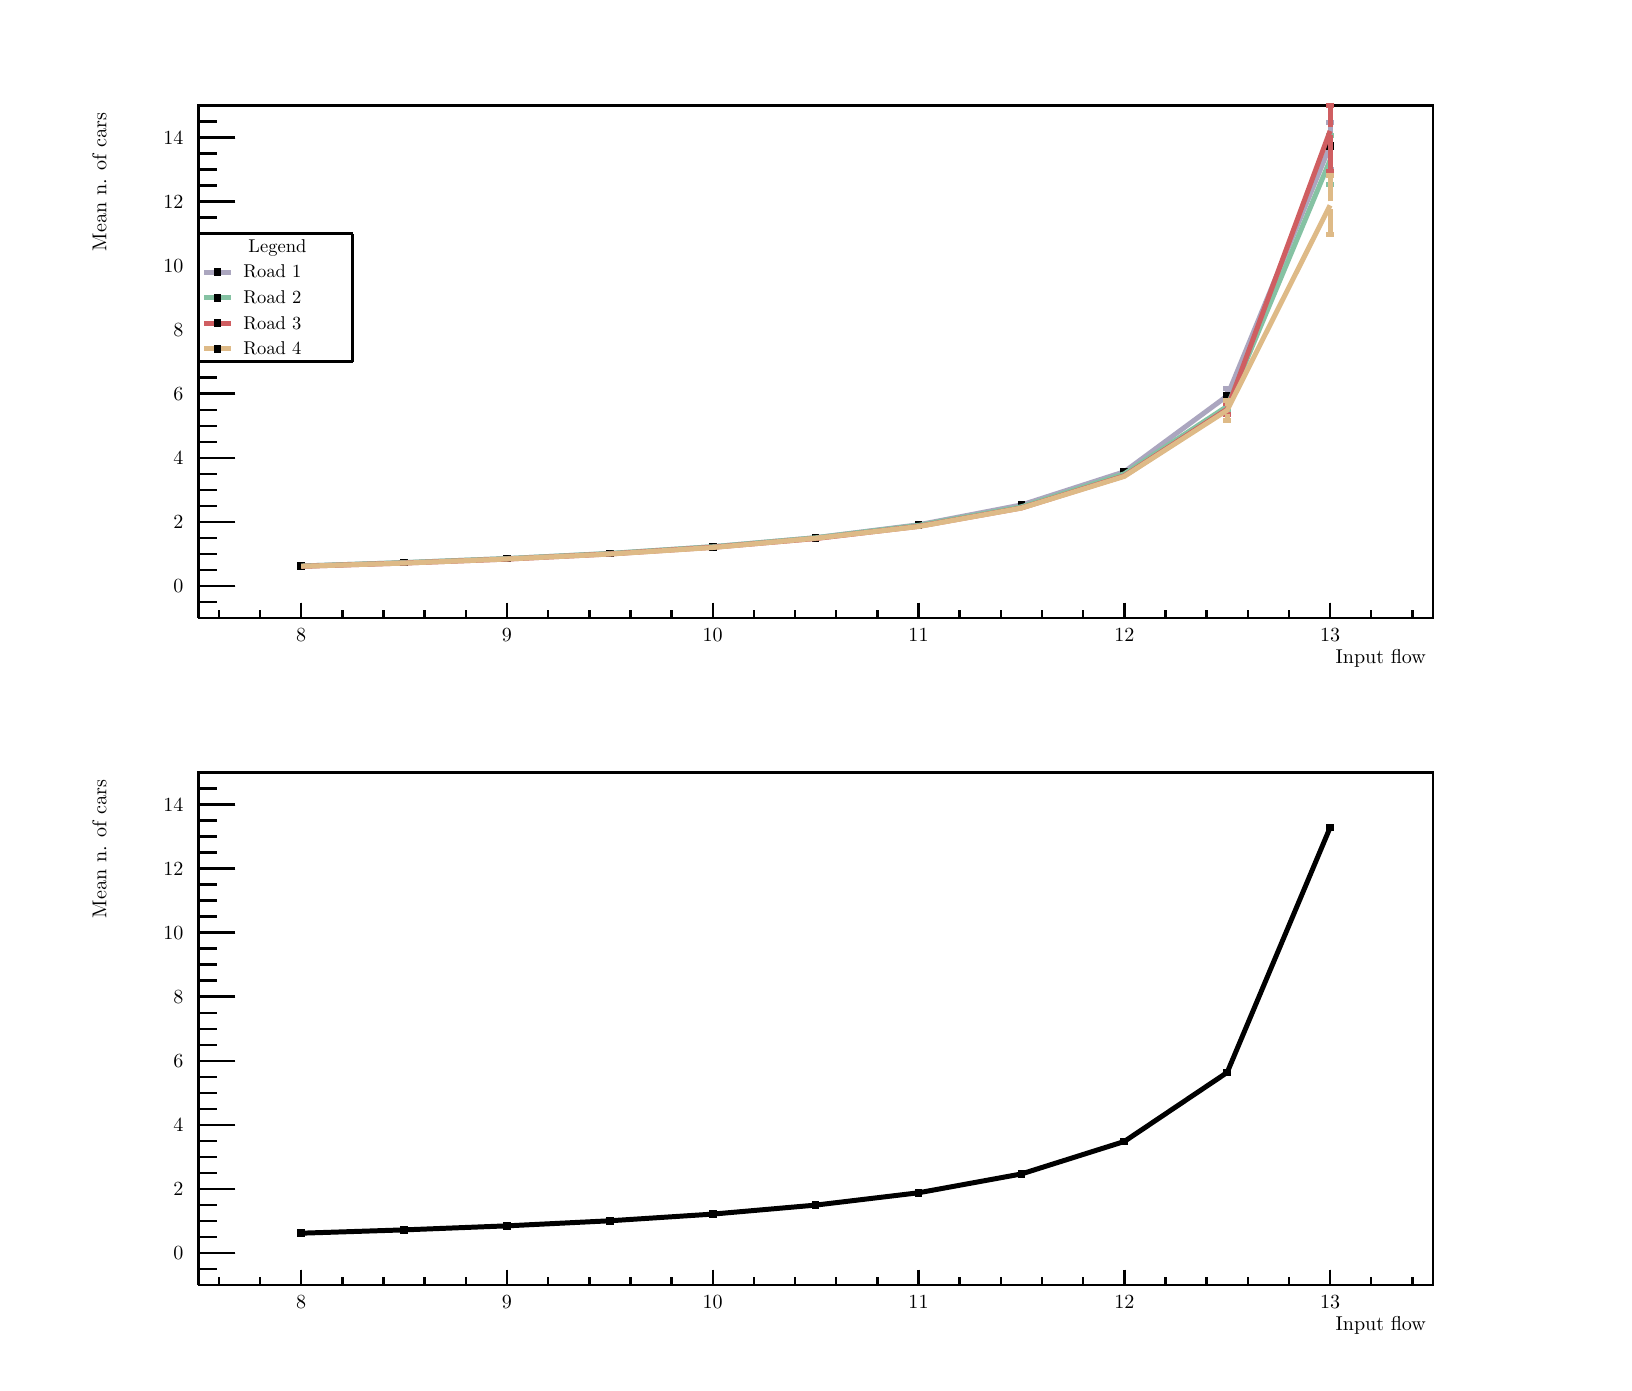
\begin{tikzpicture}
\def\CheckTikzLibraryLoaded#1{ \ifcsname tikz@library@#1@loaded\endcsname \else \PackageWarning{tikz}{usetikzlibrary{#1} is missing in the preamble.} \fi }
\CheckTikzLibraryLoaded{patterns}
\CheckTikzLibraryLoaded{plotmarks}
\pgfdeclareplotmark{cross} {
\pgfpathmoveto{\pgfpoint{-0.3\pgfplotmarksize}{\pgfplotmarksize}}
\pgfpathlineto{\pgfpoint{+0.3\pgfplotmarksize}{\pgfplotmarksize}}
\pgfpathlineto{\pgfpoint{+0.3\pgfplotmarksize}{0.3\pgfplotmarksize}}
\pgfpathlineto{\pgfpoint{+1\pgfplotmarksize}{0.3\pgfplotmarksize}}
\pgfpathlineto{\pgfpoint{+1\pgfplotmarksize}{-0.3\pgfplotmarksize}}
\pgfpathlineto{\pgfpoint{+0.3\pgfplotmarksize}{-0.3\pgfplotmarksize}}
\pgfpathlineto{\pgfpoint{+0.3\pgfplotmarksize}{-1.\pgfplotmarksize}}
\pgfpathlineto{\pgfpoint{-0.3\pgfplotmarksize}{-1.\pgfplotmarksize}}
\pgfpathlineto{\pgfpoint{-0.3\pgfplotmarksize}{-0.3\pgfplotmarksize}}
\pgfpathlineto{\pgfpoint{-1.\pgfplotmarksize}{-0.3\pgfplotmarksize}}
\pgfpathlineto{\pgfpoint{-1.\pgfplotmarksize}{0.3\pgfplotmarksize}}
\pgfpathlineto{\pgfpoint{-0.3\pgfplotmarksize}{0.3\pgfplotmarksize}}
\pgfpathclose
\pgfusepathqstroke
}
\pgfdeclareplotmark{cross*} {
\pgfpathmoveto{\pgfpoint{-0.3\pgfplotmarksize}{\pgfplotmarksize}}
\pgfpathlineto{\pgfpoint{+0.3\pgfplotmarksize}{\pgfplotmarksize}}
\pgfpathlineto{\pgfpoint{+0.3\pgfplotmarksize}{0.3\pgfplotmarksize}}
\pgfpathlineto{\pgfpoint{+1\pgfplotmarksize}{0.3\pgfplotmarksize}}
\pgfpathlineto{\pgfpoint{+1\pgfplotmarksize}{-0.3\pgfplotmarksize}}
\pgfpathlineto{\pgfpoint{+0.3\pgfplotmarksize}{-0.3\pgfplotmarksize}}
\pgfpathlineto{\pgfpoint{+0.3\pgfplotmarksize}{-1.\pgfplotmarksize}}
\pgfpathlineto{\pgfpoint{-0.3\pgfplotmarksize}{-1.\pgfplotmarksize}}
\pgfpathlineto{\pgfpoint{-0.3\pgfplotmarksize}{-0.3\pgfplotmarksize}}
\pgfpathlineto{\pgfpoint{-1.\pgfplotmarksize}{-0.3\pgfplotmarksize}}
\pgfpathlineto{\pgfpoint{-1.\pgfplotmarksize}{0.3\pgfplotmarksize}}
\pgfpathlineto{\pgfpoint{-0.3\pgfplotmarksize}{0.3\pgfplotmarksize}}
\pgfpathclose
\pgfusepathqfillstroke
}
\pgfdeclareplotmark{newstar} {
\pgfpathmoveto{\pgfqpoint{0pt}{\pgfplotmarksize}}
\pgfpathlineto{\pgfqpointpolar{44}{0.5\pgfplotmarksize}}
\pgfpathlineto{\pgfqpointpolar{18}{\pgfplotmarksize}}
\pgfpathlineto{\pgfqpointpolar{-20}{0.5\pgfplotmarksize}}
\pgfpathlineto{\pgfqpointpolar{-54}{\pgfplotmarksize}}
\pgfpathlineto{\pgfqpointpolar{-90}{0.5\pgfplotmarksize}}
\pgfpathlineto{\pgfqpointpolar{234}{\pgfplotmarksize}}
\pgfpathlineto{\pgfqpointpolar{198}{0.5\pgfplotmarksize}}
\pgfpathlineto{\pgfqpointpolar{162}{\pgfplotmarksize}}
\pgfpathlineto{\pgfqpointpolar{134}{0.5\pgfplotmarksize}}
\pgfpathclose
\pgfusepathqstroke
}
\pgfdeclareplotmark{newstar*} {
\pgfpathmoveto{\pgfqpoint{0pt}{\pgfplotmarksize}}
\pgfpathlineto{\pgfqpointpolar{44}{0.5\pgfplotmarksize}}
\pgfpathlineto{\pgfqpointpolar{18}{\pgfplotmarksize}}
\pgfpathlineto{\pgfqpointpolar{-20}{0.5\pgfplotmarksize}}
\pgfpathlineto{\pgfqpointpolar{-54}{\pgfplotmarksize}}
\pgfpathlineto{\pgfqpointpolar{-90}{0.5\pgfplotmarksize}}
\pgfpathlineto{\pgfqpointpolar{234}{\pgfplotmarksize}}
\pgfpathlineto{\pgfqpointpolar{198}{0.5\pgfplotmarksize}}
\pgfpathlineto{\pgfqpointpolar{162}{\pgfplotmarksize}}
\pgfpathlineto{\pgfqpointpolar{134}{0.5\pgfplotmarksize}}
\pgfpathclose
\pgfusepathqfillstroke
}
\definecolor{c}{rgb}{1,1,1};
\draw [color=c, fill=c] (0,0) rectangle (20,16.9424);
\draw [color=c, fill=c] (0.2,8.6406) rectangle (19.8,16.7729);
\draw [color=c, fill=c] (2.16,9.45383) rectangle (17.84,15.9597);
\definecolor{c}{rgb}{0,0,0};
\draw [c,line width=0.9] (2.16,9.45383) -- (2.16,15.9597) -- (17.84,15.9597) -- (17.84,9.45383) -- (2.16,9.45383);
\definecolor{c}{rgb}{1,1,1};
\draw [color=c, fill=c] (2.16,9.45383) rectangle (17.84,15.9597);
\definecolor{c}{rgb}{0,0,0};
\draw [c,line width=0.9] (2.16,9.45383) -- (2.16,15.9597) -- (17.84,15.9597) -- (17.84,9.45383) -- (2.16,9.45383);
\draw [c,line width=0.9] (2.16,9.45383) -- (17.84,9.45383);
\draw [c,line width=0.9] (3.46667,9.64901) -- (3.46667,9.45383);
\draw [c,line width=0.9] (3.98933,9.55142) -- (3.98933,9.45383);
\draw [c,line width=0.9] (4.512,9.55142) -- (4.512,9.45383);
\draw [c,line width=0.9] (5.03467,9.55142) -- (5.03467,9.45383);
\draw [c,line width=0.9] (5.55733,9.55142) -- (5.55733,9.45383);
\draw [c,line width=0.9] (6.08,9.64901) -- (6.08,9.45383);
\draw [c,line width=0.9] (6.60267,9.55142) -- (6.60267,9.45383);
\draw [c,line width=0.9] (7.12533,9.55142) -- (7.12533,9.45383);
\draw [c,line width=0.9] (7.648,9.55142) -- (7.648,9.45383);
\draw [c,line width=0.9] (8.17067,9.55142) -- (8.17067,9.45383);
\draw [c,line width=0.9] (8.69333,9.64901) -- (8.69333,9.45383);
\draw [c,line width=0.9] (9.216,9.55142) -- (9.216,9.45383);
\draw [c,line width=0.9] (9.73867,9.55142) -- (9.73867,9.45383);
\draw [c,line width=0.9] (10.2613,9.55142) -- (10.2613,9.45383);
\draw [c,line width=0.9] (10.784,9.55142) -- (10.784,9.45383);
\draw [c,line width=0.9] (11.3067,9.64901) -- (11.3067,9.45383);
\draw [c,line width=0.9] (11.8293,9.55142) -- (11.8293,9.45383);
\draw [c,line width=0.9] (12.352,9.55142) -- (12.352,9.45383);
\draw [c,line width=0.9] (12.8747,9.55142) -- (12.8747,9.45383);
\draw [c,line width=0.9] (13.3973,9.55142) -- (13.3973,9.45383);
\draw [c,line width=0.9] (13.92,9.64901) -- (13.92,9.45383);
\draw [c,line width=0.9] (14.4427,9.55142) -- (14.4427,9.45383);
\draw [c,line width=0.9] (14.9653,9.55142) -- (14.9653,9.45383);
\draw [c,line width=0.9] (15.488,9.55142) -- (15.488,9.45383);
\draw [c,line width=0.9] (16.0107,9.55142) -- (16.0107,9.45383);
\draw [c,line width=0.9] (16.5333,9.64901) -- (16.5333,9.45383);
\draw [c,line width=0.9] (3.46667,9.64901) -- (3.46667,9.45383);
\draw [c,line width=0.9] (2.944,9.55142) -- (2.944,9.45383);
\draw [c,line width=0.9] (2.42133,9.55142) -- (2.42133,9.45383);
\draw [c,line width=0.9] (16.5333,9.64901) -- (16.5333,9.45383);
\draw [c,line width=0.9] (17.056,9.55142) -- (17.056,9.45383);
\draw [c,line width=0.9] (17.5787,9.55142) -- (17.5787,9.45383);
\draw [anchor=base] (3.46667,9.15294) node[scale=0.724696, color=c, rotate=0]{8};
\draw [anchor=base] (6.08,9.15294) node[scale=0.724696, color=c, rotate=0]{9};
\draw [anchor=base] (8.69333,9.15294) node[scale=0.724696, color=c, rotate=0]{10};
\draw [anchor=base] (11.3067,9.15294) node[scale=0.724696, color=c, rotate=0]{11};
\draw [anchor=base] (13.92,9.15294) node[scale=0.724696, color=c, rotate=0]{12};
\draw [anchor=base] (16.5333,9.15294) node[scale=0.724696, color=c, rotate=0]{13};
\draw [anchor= east] (17.84,8.93337) node[scale=0.724696, color=c, rotate=0]{Input flow};
\draw [c,line width=0.9] (2.16,9.45383) -- (2.16,15.9597);
\draw [c,line width=0.9] (2.6304,9.86045) -- (2.16,9.86045);
\draw [c,line width=0.9] (2.3952,10.0638) -- (2.16,10.0638);
\draw [c,line width=0.9] (2.3952,10.2671) -- (2.16,10.2671);
\draw [c,line width=0.9] (2.3952,10.4704) -- (2.16,10.4704);
\draw [c,line width=0.9] (2.6304,10.6737) -- (2.16,10.6737);
\draw [c,line width=0.9] (2.3952,10.877) -- (2.16,10.877);
\draw [c,line width=0.9] (2.3952,11.0803) -- (2.16,11.0803);
\draw [c,line width=0.9] (2.3952,11.2836) -- (2.16,11.2836);
\draw [c,line width=0.9] (2.6304,11.4869) -- (2.16,11.4869);
\draw [c,line width=0.9] (2.3952,11.6902) -- (2.16,11.6902);
\draw [c,line width=0.9] (2.3952,11.8935) -- (2.16,11.8935);
\draw [c,line width=0.9] (2.3952,12.0968) -- (2.16,12.0968);
\draw [c,line width=0.9] (2.6304,12.3002) -- (2.16,12.3002);
\draw [c,line width=0.9] (2.3952,12.5035) -- (2.16,12.5035);
\draw [c,line width=0.9] (2.3952,12.7068) -- (2.16,12.7068);
\draw [c,line width=0.9] (2.3952,12.9101) -- (2.16,12.9101);
\draw [c,line width=0.9] (2.6304,13.1134) -- (2.16,13.1134);
\draw [c,line width=0.9] (2.3952,13.3167) -- (2.16,13.3167);
\draw [c,line width=0.9] (2.3952,13.52) -- (2.16,13.52);
\draw [c,line width=0.9] (2.3952,13.7233) -- (2.16,13.7233);
\draw [c,line width=0.9] (2.6304,13.9266) -- (2.16,13.9266);
\draw [c,line width=0.9] (2.3952,14.1299) -- (2.16,14.1299);
\draw [c,line width=0.9] (2.3952,14.3332) -- (2.16,14.3332);
\draw [c,line width=0.9] (2.3952,14.5365) -- (2.16,14.5365);
\draw [c,line width=0.9] (2.6304,14.7399) -- (2.16,14.7399);
\draw [c,line width=0.9] (2.3952,14.9432) -- (2.16,14.9432);
\draw [c,line width=0.9] (2.3952,15.1465) -- (2.16,15.1465);
\draw [c,line width=0.9] (2.3952,15.3498) -- (2.16,15.3498);
\draw [c,line width=0.9] (2.6304,15.5531) -- (2.16,15.5531);
\draw [c,line width=0.9] (2.6304,9.86045) -- (2.16,9.86045);
\draw [c,line width=0.9] (2.3952,9.65714) -- (2.16,9.65714);
\draw [c,line width=0.9] (2.3952,9.45383) -- (2.16,9.45383);
\draw [c,line width=0.9] (2.6304,15.5531) -- (2.16,15.5531);
\draw [c,line width=0.9] (2.3952,15.7564) -- (2.16,15.7564);
\draw [c,line width=0.9] (2.3952,15.9597) -- (2.16,15.9597);
\draw [anchor= east] (2.062,9.86045) node[scale=0.724696, color=c, rotate=0]{0};
\draw [anchor= east] (2.062,10.6737) node[scale=0.724696, color=c, rotate=0]{2};
\draw [anchor= east] (2.062,11.4869) node[scale=0.724696, color=c, rotate=0]{4};
\draw [anchor= east] (2.062,12.3002) node[scale=0.724696, color=c, rotate=0]{6};
\draw [anchor= east] (2.062,13.1134) node[scale=0.724696, color=c, rotate=0]{8};
\draw [anchor= east] (2.062,13.9266) node[scale=0.724696, color=c, rotate=0]{10};
\draw [anchor= east] (2.062,14.7399) node[scale=0.724696, color=c, rotate=0]{12};
\draw [anchor= east] (2.062,15.5531) node[scale=0.724696, color=c, rotate=0]{14};
\draw [anchor= east] (0.9056,15.9597) node[scale=0.724696, color=c, rotate=90]{Mean n. of cars};
\definecolor{c}{rgb}{0.67,0.65,0.75};
\draw [c,line width=1.8] (3.46667,10.1128) -- (4.77333,10.1548) -- (6.08,10.207) -- (7.38667,10.2704) -- (8.69333,10.3573) -- (10,10.4719) -- (11.3067,10.6359) -- (12.6133,10.8879) -- (13.92,11.3091) -- (15.2267,12.2722) -- (16.5333,15.4493);
\definecolor{c}{rgb}{0,0,0};
\foreach \P in {(3.46667,10.1128), (4.77333,10.1548), (6.08,10.207), (7.38667,10.2704), (8.69333,10.3573), (10,10.4719), (11.3067,10.6359), (12.6133,10.8879), (13.92,11.3091), (15.2267,12.2722), (16.5333,15.4493)}{\draw[mark
 options={color=c,fill=c},mark size=1.201201pt, line width=0.000000pt, mark=square*] plot coordinates {\P};}
\definecolor{c}{rgb}{0.67,0.65,0.75};
\draw [c,line width=1.8] (15.2267,12.3223) -- (15.2267,12.3727);
\draw [c,line width=1.8] (15.1765,12.3727) -- (15.2768,12.3727);
\draw [c,line width=1.8] (15.2267,12.2221) -- (15.2267,12.1718);
\draw [c,line width=1.8] (15.1765,12.1718) -- (15.2768,12.1718);
\draw [c,line width=1.8] (16.5333,15.4994) -- (16.5333,15.7445);
\draw [c,line width=1.8] (16.4832,15.7445) -- (16.5835,15.7445);
\draw [c,line width=1.8] (16.5333,15.3991) -- (16.5333,15.154);
\draw [c,line width=1.8] (16.4832,15.154) -- (16.5835,15.154);
\definecolor{c}{rgb}{0.52,0.76,0.64};
\draw [c,line width=1.8] (15.2267,12.1906) -- (15.2267,12.2106);
\draw [c,line width=1.8] (15.1765,12.2106) -- (15.2768,12.2106);
\draw [c,line width=1.8] (15.2267,12.0903) -- (15.2267,12.0703);
\draw [c,line width=1.8] (15.1765,12.0703) -- (15.2768,12.0703);
\draw [c,line width=1.8] (16.5333,15.3156) -- (16.5333,15.5781);
\draw [c,line width=1.8] (16.4832,15.5781) -- (16.5835,15.5781);
\draw [c,line width=1.8] (16.5333,15.2154) -- (16.5333,14.9529);
\draw [c,line width=1.8] (16.4832,14.9529) -- (16.5835,14.9529);
\draw [c,line width=1.8] (3.46667,10.1121) -- (4.77333,10.156) -- (6.08,10.2068) -- (7.38667,10.2722) -- (8.69333,10.3572) -- (10,10.4711) -- (11.3067,10.6288) -- (12.6133,10.8655) -- (13.92,11.2836) -- (15.2267,12.1404) -- (16.5333,15.2655);
\definecolor{c}{rgb}{0.81,0.37,0.38};
\draw [c,line width=1.8] (15.2267,12.1551) -- (15.2267,12.1781);
\draw [c,line width=1.8] (15.1765,12.1781) -- (15.2768,12.1781);
\draw [c,line width=1.8] (15.2267,12.0549) -- (15.2267,12.0319);
\draw [c,line width=1.8] (15.1765,12.0319) -- (15.2768,12.0319);
\draw [c,line width=1.8] (16.5333,15.6878) -- (16.5333,15.9597);
\draw [c,line width=1.8] (16.4832,15.9597) -- (16.5835,15.9597);
\draw [c,line width=1.8] (16.5333,15.5876) -- (16.5333,15.1272);
\draw [c,line width=1.8] (16.4832,15.1272) -- (16.5835,15.1272);
\draw [c,line width=1.8] (3.46667,10.108) -- (4.77333,10.1499) -- (6.08,10.2) -- (7.38667,10.2656) -- (8.69333,10.3499) -- (10,10.4612) -- (11.3067,10.6163) -- (12.6133,10.8498) -- (13.92,11.2567) -- (15.2267,12.105) -- (16.5333,15.6377);
\definecolor{c}{rgb}{0.87,0.73,0.53};
\draw [c,line width=1.8] (15.2267,12.1411) -- (15.2267,12.2159);
\draw [c,line width=1.8] (15.1765,12.2159) -- (15.2768,12.2159);
\draw [c,line width=1.8] (15.2267,12.0409) -- (15.2267,11.9661);
\draw [c,line width=1.8] (15.1765,11.9661) -- (15.2768,11.9661);
\draw [c,line width=1.8] (16.5333,14.7434) -- (16.5333,15.0698);
\draw [c,line width=1.8] (16.4832,15.0698) -- (16.5835,15.0698);
\draw [c,line width=1.8] (16.5333,14.6431) -- (16.5333,14.3167);
\draw [c,line width=1.8] (16.4832,14.3167) -- (16.5835,14.3167);
\draw [c,line width=1.8] (3.46667,10.1087) -- (4.77333,10.1491) -- (6.08,10.2011) -- (7.38667,10.2641) -- (8.69333,10.3473) -- (10,10.4643) -- (11.3067,10.6137) -- (12.6133,10.848) -- (13.92,11.2507) -- (15.2267,12.091) -- (16.5333,14.6933);
\definecolor{c}{rgb}{1,1,1};
\draw [color=c, fill=c] (2.16,12.7068) rectangle (4.12,14.3332);
\definecolor{c}{rgb}{0,0,0};
\draw [c,line width=0.9] (2.16,12.7068) -- (4.12,12.7068);
\draw [c,line width=0.9] (4.12,12.7068) -- (4.12,14.3332);
\draw [c,line width=0.9] (4.12,14.3332) -- (2.16,14.3332);
\draw [c,line width=0.9] (2.16,14.3332) -- (2.16,12.7068);
\draw [anchor=base] (3.1645,14.0974) node[scale=0.66895, color=c, rotate=0]{Legend};
\draw [anchor=base west] (2.65,13.7721) node[scale=0.66895, color=c, rotate=0]{Road 1};
\definecolor{c}{rgb}{1,1,1};
\draw [c, fill=c] (2.2335,13.7314) -- (2.5765,13.7314) -- (2.5765,13.9591) -- (2.2335,13.9591);
\definecolor{c}{rgb}{0.67,0.65,0.75};
\draw [c,line width=1.8] (2.2335,13.8453) -- (2.5765,13.8453);
\definecolor{c}{rgb}{0,0,0};
\foreach \P in {(2.405,13.8453)}{\draw[mark options={color=c,fill=c},mark size=1.201201pt, line width=0.000000pt, mark=square*] plot coordinates {\P};}
\draw [anchor=base west] (2.65,13.4468) node[scale=0.66895, color=c, rotate=0]{Road 2};
\definecolor{c}{rgb}{1,1,1};
\draw [c, fill=c] (2.2335,13.4061) -- (2.5765,13.4061) -- (2.5765,13.6339) -- (2.2335,13.6339);
\definecolor{c}{rgb}{0.52,0.76,0.64};
\draw [c,line width=1.8] (2.2335,13.52) -- (2.5765,13.52);
\definecolor{c}{rgb}{0,0,0};
\foreach \P in {(2.405,13.52)}{\draw[mark options={color=c,fill=c},mark size=1.201201pt, line width=0.000000pt, mark=square*] plot coordinates {\P};}
\draw [anchor=base west] (2.65,13.1215) node[scale=0.66895, color=c, rotate=0]{Road 3};
\definecolor{c}{rgb}{1,1,1};
\draw [c, fill=c] (2.2335,13.0809) -- (2.5765,13.0809) -- (2.5765,13.3086) -- (2.2335,13.3086);
\definecolor{c}{rgb}{0.81,0.37,0.38};
\draw [c,line width=1.8] (2.2335,13.1947) -- (2.5765,13.1947);
\definecolor{c}{rgb}{0,0,0};
\foreach \P in {(2.405,13.1947)}{\draw[mark options={color=c,fill=c},mark size=1.201201pt, line width=0.000000pt, mark=square*] plot coordinates {\P};}
\draw [anchor=base west] (2.65,12.7962) node[scale=0.66895, color=c, rotate=0]{Road 4};
\definecolor{c}{rgb}{1,1,1};
\draw [c, fill=c] (2.2335,12.7556) -- (2.5765,12.7556) -- (2.5765,12.9833) -- (2.2335,12.9833);
\definecolor{c}{rgb}{0.87,0.73,0.53};
\draw [c,line width=1.8] (2.2335,12.8694) -- (2.5765,12.8694);
\definecolor{c}{rgb}{0,0,0};
\foreach \P in {(2.405,12.8694)}{\draw[mark options={color=c,fill=c},mark size=1.201201pt, line width=0.000000pt, mark=square*] plot coordinates {\P};}
\definecolor{c}{rgb}{1,1,1};
\draw [color=c, fill=c] (0.2,0.169424) rectangle (19.8,8.30175);
\draw [color=c, fill=c] (2.16,0.982657) rectangle (17.84,7.48852);
\definecolor{c}{rgb}{0,0,0};
\draw [c,line width=0.9] (2.16,0.982657) -- (2.16,7.48852) -- (17.84,7.48852) -- (17.84,0.982657) -- (2.16,0.982657);
\definecolor{c}{rgb}{1,1,1};
\draw [color=c, fill=c] (2.16,0.982657) rectangle (17.84,7.48852);
\definecolor{c}{rgb}{0,0,0};
\draw [c,line width=0.9] (2.16,0.982657) -- (2.16,7.48852) -- (17.84,7.48852) -- (17.84,0.982657) -- (2.16,0.982657);
\draw [c,line width=0.9] (2.16,0.982657) -- (17.84,0.982657);
\draw [c,line width=0.9] (3.46667,1.17783) -- (3.46667,0.982657);
\draw [c,line width=0.9] (3.98933,1.08024) -- (3.98933,0.982657);
\draw [c,line width=0.9] (4.512,1.08024) -- (4.512,0.982657);
\draw [c,line width=0.9] (5.03467,1.08024) -- (5.03467,0.982657);
\draw [c,line width=0.9] (5.55733,1.08024) -- (5.55733,0.982657);
\draw [c,line width=0.9] (6.08,1.17783) -- (6.08,0.982657);
\draw [c,line width=0.9] (6.60267,1.08024) -- (6.60267,0.982657);
\draw [c,line width=0.9] (7.12533,1.08024) -- (7.12533,0.982657);
\draw [c,line width=0.9] (7.648,1.08024) -- (7.648,0.982657);
\draw [c,line width=0.9] (8.17067,1.08024) -- (8.17067,0.982657);
\draw [c,line width=0.9] (8.69333,1.17783) -- (8.69333,0.982657);
\draw [c,line width=0.9] (9.216,1.08024) -- (9.216,0.982657);
\draw [c,line width=0.9] (9.73867,1.08024) -- (9.73867,0.982657);
\draw [c,line width=0.9] (10.2613,1.08024) -- (10.2613,0.982657);
\draw [c,line width=0.9] (10.784,1.08024) -- (10.784,0.982657);
\draw [c,line width=0.9] (11.3067,1.17783) -- (11.3067,0.982657);
\draw [c,line width=0.9] (11.8293,1.08024) -- (11.8293,0.982657);
\draw [c,line width=0.9] (12.352,1.08024) -- (12.352,0.982657);
\draw [c,line width=0.9] (12.8747,1.08024) -- (12.8747,0.982657);
\draw [c,line width=0.9] (13.3973,1.08024) -- (13.3973,0.982657);
\draw [c,line width=0.9] (13.92,1.17783) -- (13.92,0.982657);
\draw [c,line width=0.9] (14.4427,1.08024) -- (14.4427,0.982657);
\draw [c,line width=0.9] (14.9653,1.08024) -- (14.9653,0.982657);
\draw [c,line width=0.9] (15.488,1.08024) -- (15.488,0.982657);
\draw [c,line width=0.9] (16.0107,1.08024) -- (16.0107,0.982657);
\draw [c,line width=0.9] (16.5333,1.17783) -- (16.5333,0.982657);
\draw [c,line width=0.9] (3.46667,1.17783) -- (3.46667,0.982657);
\draw [c,line width=0.9] (2.944,1.08024) -- (2.944,0.982657);
\draw [c,line width=0.9] (2.42133,1.08024) -- (2.42133,0.982657);
\draw [c,line width=0.9] (16.5333,1.17783) -- (16.5333,0.982657);
\draw [c,line width=0.9] (17.056,1.08024) -- (17.056,0.982657);
\draw [c,line width=0.9] (17.5787,1.08024) -- (17.5787,0.982657);
\draw [anchor=base] (3.46667,0.68176) node[scale=0.724696, color=c, rotate=0]{8};
\draw [anchor=base] (6.08,0.68176) node[scale=0.724696, color=c, rotate=0]{9};
\draw [anchor=base] (8.69333,0.68176) node[scale=0.724696, color=c, rotate=0]{10};
\draw [anchor=base] (11.3067,0.68176) node[scale=0.724696, color=c, rotate=0]{11};
\draw [anchor=base] (13.92,0.68176) node[scale=0.724696, color=c, rotate=0]{12};
\draw [anchor=base] (16.5333,0.68176) node[scale=0.724696, color=c, rotate=0]{13};
\draw [anchor= east] (17.84,0.462188) node[scale=0.724696, color=c, rotate=0]{Input flow};
\draw [c,line width=0.9] (2.16,0.982657) -- (2.16,7.48852);
\draw [c,line width=0.9] (2.6304,1.38927) -- (2.16,1.38927);
\draw [c,line width=0.9] (2.3952,1.59258) -- (2.16,1.59258);
\draw [c,line width=0.9] (2.3952,1.79589) -- (2.16,1.79589);
\draw [c,line width=0.9] (2.3952,1.9992) -- (2.16,1.9992);
\draw [c,line width=0.9] (2.6304,2.20251) -- (2.16,2.20251);
\draw [c,line width=0.9] (2.3952,2.40581) -- (2.16,2.40581);
\draw [c,line width=0.9] (2.3952,2.60912) -- (2.16,2.60912);
\draw [c,line width=0.9] (2.3952,2.81243) -- (2.16,2.81243);
\draw [c,line width=0.9] (2.6304,3.01574) -- (2.16,3.01574);
\draw [c,line width=0.9] (2.3952,3.21905) -- (2.16,3.21905);
\draw [c,line width=0.9] (2.3952,3.42236) -- (2.16,3.42236);
\draw [c,line width=0.9] (2.3952,3.62566) -- (2.16,3.62566);
\draw [c,line width=0.9] (2.6304,3.82897) -- (2.16,3.82897);
\draw [c,line width=0.9] (2.3952,4.03228) -- (2.16,4.03228);
\draw [c,line width=0.9] (2.3952,4.23559) -- (2.16,4.23559);
\draw [c,line width=0.9] (2.3952,4.4389) -- (2.16,4.4389);
\draw [c,line width=0.9] (2.6304,4.64221) -- (2.16,4.64221);
\draw [c,line width=0.9] (2.3952,4.84551) -- (2.16,4.84551);
\draw [c,line width=0.9] (2.3952,5.04882) -- (2.16,5.04882);
\draw [c,line width=0.9] (2.3952,5.25213) -- (2.16,5.25213);
\draw [c,line width=0.9] (2.6304,5.45544) -- (2.16,5.45544);
\draw [c,line width=0.9] (2.3952,5.65875) -- (2.16,5.65875);
\draw [c,line width=0.9] (2.3952,5.86206) -- (2.16,5.86206);
\draw [c,line width=0.9] (2.3952,6.06536) -- (2.16,6.06536);
\draw [c,line width=0.9] (2.6304,6.26867) -- (2.16,6.26867);
\draw [c,line width=0.9] (2.3952,6.47198) -- (2.16,6.47198);
\draw [c,line width=0.9] (2.3952,6.67529) -- (2.16,6.67529);
\draw [c,line width=0.9] (2.3952,6.8786) -- (2.16,6.8786);
\draw [c,line width=0.9] (2.6304,7.0819) -- (2.16,7.0819);
\draw [c,line width=0.9] (2.6304,1.38927) -- (2.16,1.38927);
\draw [c,line width=0.9] (2.3952,1.18596) -- (2.16,1.18596);
\draw [c,line width=0.9] (2.3952,0.982657) -- (2.16,0.982657);
\draw [c,line width=0.9] (2.6304,7.0819) -- (2.16,7.0819);
\draw [c,line width=0.9] (2.3952,7.28521) -- (2.16,7.28521);
\draw [c,line width=0.9] (2.3952,7.48852) -- (2.16,7.48852);
\draw [anchor= east] (2.062,1.38927) node[scale=0.724696, color=c, rotate=0]{0};
\draw [anchor= east] (2.062,2.20251) node[scale=0.724696, color=c, rotate=0]{2};
\draw [anchor= east] (2.062,3.01574) node[scale=0.724696, color=c, rotate=0]{4};
\draw [anchor= east] (2.062,3.82897) node[scale=0.724696, color=c, rotate=0]{6};
\draw [anchor= east] (2.062,4.64221) node[scale=0.724696, color=c, rotate=0]{8};
\draw [anchor= east] (2.062,5.45544) node[scale=0.724696, color=c, rotate=0]{10};
\draw [anchor= east] (2.062,6.26867) node[scale=0.724696, color=c, rotate=0]{12};
\draw [anchor= east] (2.062,7.0819) node[scale=0.724696, color=c, rotate=0]{14};
\draw [anchor= east] (0.9056,7.48852) node[scale=0.724696, color=c, rotate=90]{Mean n. of cars};
\draw [c,line width=1.8] (3.46667,1.6392) -- (4.77333,1.68126) -- (6.08,1.73255) -- (7.38667,1.79691) -- (8.69333,1.88176) -- (10,1.99595) -- (11.3067,2.15249) -- (12.6133,2.39162) -- (13.92,2.80386) -- (15.2267,3.68099) -- (16.5333,6.79025);
\foreach \P in {(3.46667,1.6392), (4.77333,1.68126), (6.08,1.73255), (7.38667,1.79691), (8.69333,1.88176), (10,1.99595), (11.3067,2.15249), (12.6133,2.39162), (13.92,2.80386), (15.2267,3.68099), (16.5333,6.79025)}{\draw[mark
 options={color=c,fill=c},mark size=1.201201pt, line width=0.000000pt, mark=square*] plot coordinates {\P};}
\end{tikzpicture}
%\end{document}
